\documentclass[12pt]{article}
\setlength\parindent{0pt}
\usepackage{fullpage}
\usepackage{amsmath}
\usepackage{graphicx}
\usepackage{tikz}
\setlength{\parskip}{4mm}
\usepackage[left=2cm, right=2cm, top=1.5cm, bottom=1cm]{geometry}
%\usepackage[margin=0.5in, paperwidth=13.5in, paperheight=8.4375in]{geometry}
\def\LL{\left\langle}   % left angle bracket
\def\RR{\right\rangle}  % right angle bracket
\def\LP{\left(}         % left parenthesis
\def\RP{\right)}        % right parenthesis
\def\LB{\left\{}        % left curly bracket
\def\RB{\right\}}       % right curly bracket
\def\PAR#1#2{ {{\partial #1}\over{\partial #2}} }
\def\PARTWO#1#2{ {{\partial^2 #1}\over{\partial #2}^2} }
\def\PARTWOMIX#1#2#3{ {{\partial^2 #1}\over{\partial #2 \partial #3}} }
\newcommand{\BI}{\begin{itemize}}
\newcommand{\EI}{\end{itemize}}
\newcommand{\BE}{\begin{displaymath}}
\newcommand{\EE}{\end{displaymath}}
\newcommand{\BNE}{\begin{equation}}
\newcommand{\ENE}{\end{equation}}
\newcommand{\BEA}{\begin{eqnarray}}
\newcommand{\EEA}{\nonumber\end{eqnarray}}
\newcommand{\EL}{\nonumber\\}
\newcommand{\la}[1]{\label{#1}}
\newcommand{\ie}{{\em i.e.\ }}
\newcommand{\eg}{{\em e.\,g.\ }}
\newcommand{\cf}{cf.\ }
\newcommand{\etc}{etc.\ }
\newcommand{\Tr}{{\rm tr}}
\newcommand{\etal}{{\it et al.}}
\newcommand{\OL}[1]{\overline{#1}\ } % overline
\newcommand{\OLL}[1]{\overline{\overline{#1}}\ } % double overline
\newcommand{\OON}{\frac{1}{N}} % "one over N"
\newcommand{\OOX}[1]{\frac{1}{#1}} % "one over X"

\def\BS{\bigskip}

\begin{document}
\pagenumbering{gobble}
\Large
\centerline{\sc{Recitation Questions -- 1D Motion (part 1)}}
\normalsize
\centerline{\sc{28 January}}
\normalsize
\medskip

\BS\BS\BS


In this recitation, you will learn how to:

\BI
\item describe simple motions in words, pictures, and mathematics, and relate those descriptions to each other
\item construct algebraic representations of questions about motion
\item think carefully about how position, velocity, and acceleration relate
\EI



\centerline{\Large Question 1: Two runners}

\begin{center}
\it (This problem is simple, but it has the same template as most of the problems that you'll be doing for this unit. Take note of the steps you take to solve it; the steps will be similar for very many of the things you do in the next few weeks.)

\end{center}
\rm
Two runners, Alice and Bob, start at opposite ends of a hundred-meter long soccer pitch and sprint toward each other. Alice runs at 8 m/s and starts on the east side, while Bob runs at 6 m/s and starts at the west side. You'd like to know where they'll meet.

\begin{enumerate}

\item Draw position vs. time graphs for both runners on a single set of axes.

\begin{center}

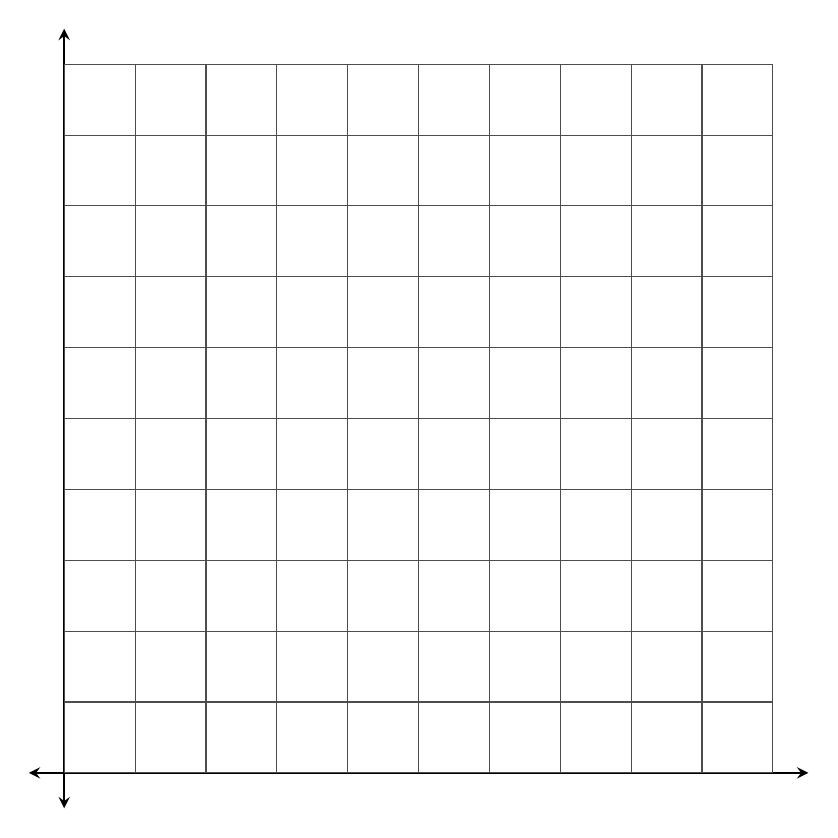
\begin{tikzpicture}[scale=0.9]
\pgfmathsetmacro{\xmin}{0}
\pgfmathsetmacro{\xmax}{10}
\pgfmathsetmacro{\ymin}{0}
\pgfmathsetmacro{\ymax}{10}

\coordinate (o) at (0,0);

\draw[thick,stealth-] (\xmin,0) +(-0.5,0) -- (\xmax,0);
\draw[thick,-stealth] (\xmax,0) -- +(0.5,0);
\draw[thick,stealth-] (0,\ymin) +(0,-0.5) -- (0,\ymax);
\draw[thick,-stealth] (0,\ymax) -- +(0,0.5);

\draw[black!70] (\xmin,\ymin) grid (\xmax, \ymax);

\end{tikzpicture}



\end{center}

\item Write position vs. time equations ($x=x_0 + vt$) for both runners. Use subscripts to distinguish their positions, \ie $x_A$ and $x_B$. Hint: Think carefully about their velocities...

\vspace{1.5in}

\item In this entire unit, the main challenge will be translating the question (``where will they meet?'') into a sentence that involves your algebraic variables. This sentence will then become your recipe for solving the problem.
Often, but not always, this will take the following form: 

\begin{center}
{\bf ``What is the value of \underline{\hspace{0.7in}} at the time when \underline{\hspace{0.7in}} is equal to \underline{\hspace{0.7in}}?''} 
\end{center}

Fill in the blanks in the above sentence to get a recipe for figuring out where the runners will meet.

\item Do the algebra indicated by your recipe and figure out where they will meet.

\vspace{2in}

\item Suppose that instead Bob had a 2 second head start. What would change in your graphs? What would change in your algebra? (Discuss in words and symbols; you don't need to do the arithmetic again.)
\end{enumerate}


\vspace{3in}
\newpage
\centerline{\Large Question 2: Motion with acceleration}

In class, you learned the kinematics relations

\begin{align*}
x(t) &= x_0 + v_0t + \frac{1}{2}at^2 \\
v(t) &= v_0 + at
\end{align*}

These relations aren't generally true, however; they are true only in a specific case. What must be true about the object's acceleration for these relations to apply?

\vspace{1.2in}
\newpage



\centerline{\Large Question 3: A bouncing basketball}

\BS

A person is holding a basketball; they drop the basketball (from rest). It falls to the ground, bounces back up, and falls back down again. Draw position vs. time, velocity vs. time, and acceleration vs. time graphs for the ball on the next page.

Look at your graphs carefully and make sure they are self-consistent:


\BI
    \item Regions of constant acceleration should correspond to places where the velocity graph is a straight line (are there any regions where the acceleration is constant? Are there any regions where it is something different?)
    \item Regions of constant velocity should correspond to places where the position graph is a straight line (are there any?)
    \item Places where the position graph is flat should correspond to $v=0$. (are there any?)
    \item Remember, the slope of the position graph is the value of the velocity graph; the slope of the velocity graph is the value of the acceleration graph. This means:
    \begin{itemize}
    	\item If the velocity is positive, the position graph should be going up
    	\item If the velocity is negative, the position graph should be going down
    	\item If the acceleration is positive, the velocity should be going up, and the position graph should be concave upwards
    	\item If the acceleration is negative, the velocity should be going down, and the position graph should be concave downwards
    \end{itemize}
\EI
     

Note: This can be quite tricky if you overthink it! As with all problems in recitation, work together with your peers and ask your TA/coach for guidance if you have questions.

\BS\BS

{\it Hint:} There is some tension here between the ``engineering reality'' of how a basketball really bounces -- where it's in contact with the ground for a measurable amount of time, during which it bounces back upward
-- and a mathematical idealization of it. You should think about a {\it real} basketball bouncing on a {\it real} floor.

\newpage


\begin{center}
	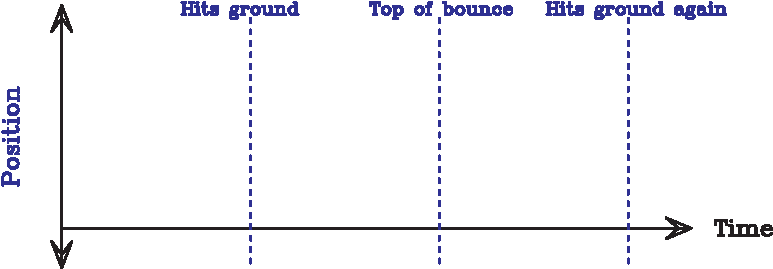
\includegraphics[width=\textwidth]{position-crop.pdf}
	
	\vspace{0.4in}
	
	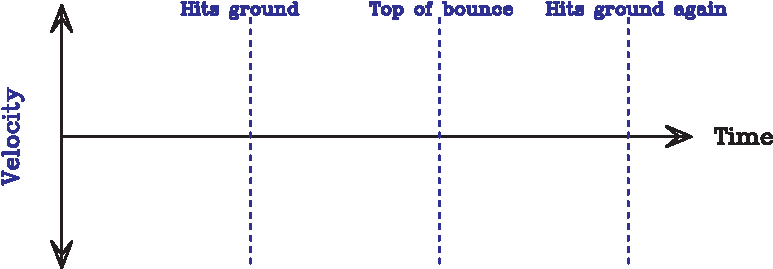
\includegraphics[width=\textwidth]{velocity-crop.pdf}
	
	\vspace{0.4in}
	
	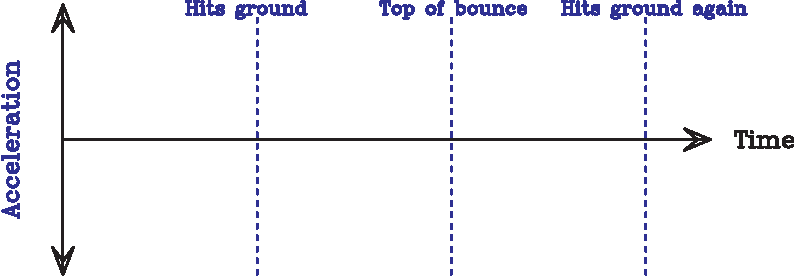
\includegraphics[width=\textwidth]{acceleration-crop.pdf}
\end{center}








\newpage


\centerline{\Large Question 4: a braking car}

A car is traveling at 30 m/s and applies its brakes to slow down to 10 m/s. If it is able to decelerate at 5 $\rm m/\rm s^2$, how far does it travel during the braking period?

\begin{enumerate}
	\item Write expressions for the car's position and velocity as a function of time. What moment makes sense to choose as your reference time $t=0$?
	
	\vspace{1in}
	
	
	\item How can you translate the question ``How far does it travel during the braking period?'' into a sentence about your algebraic variables? Again, fill in the blanks: 
	
	\begin{center}
		{\bf ``What is the value of \underline{\hspace{0.7in}} at the time when \underline{\hspace{0.7in}} is equal to \underline{\hspace{0.7in}}?''} 
	\end{center}
	
	
	\item What intermediate quantity must you find before you find the distance traveled? Following the above recipe you created for yourself, find it.
	
	
	
	
	\vspace{2in}
	
	
	
	
	
	\item Finally, how far does the car travel during the braking period?
	
	\newpage


\end{enumerate}

\end{document}
